\documentclass[a4paper,12pt,titlepage]{article}
\usepackage{amsmath} 
\usepackage{amssymb}
\usepackage[nottoc]{tocbibind}
\usepackage{float}
\usepackage{indentfirst}
\author{\textit{Jiang Yicheng}\\\textit{515370910224}}
\title{\textbf{VV286\\ Honors Mathematics IV\\
Ordinary Differential Equations\\
		Assignment 2}}
\date{\today}

\usepackage[top=1 in, bottom=0.8 in, left= 1in, right=1 in]{geometry}
\usepackage{fancyhdr,lastpage}
	\pagestyle{fancy}
	\fancyhf{}
\cfoot{Page \thepage\ of \pageref{LastPage}}
\usepackage{multirow}
\usepackage{gauss}
\usepackage{geometry}
\usepackage{graphicx}
\begin{document}

\maketitle

\section{}
\paragraph{Proof:}
Set $u(x)=e^{\int h(x)y(x)dx}$, then
\begin{equation*}
\dfrac{du}{dx}=\dfrac{d}{dx}e^{\int h(x)y(x)dx}=e^{\int h(x)y(x)dx}\cdot h(x)y(x)
\end{equation*}
\begin{align*}
\dfrac{d^2u}{dx^2}&=\dfrac{d}{dx}(e^{\int h(x)y(x)dx}\cdot h(x)y(x))\\
&=e^{\int h(x)y(x)dx}\cdot (h(x)y(x))^2+e^{\int h(x)y(x)dx}(h'(x)y(x)+h(x)y'(x))
\end{align*}
Then
\begin{align*}
&u''+\Big(g-\dfrac{h'}{h}\Big)u'-khu\\
=&e^{\int h(x)y(x)dx}\cdot (h(x)y(x))^2+e^{\int h(x)y(x)dx}(h'(x)y(x)+h(x)y'(x))\\
&+\Big(g(x)-\dfrac{h'(x)}{h(x)}\Big)e^{\int h(x)y(x)dx}\cdot h(x)y(x)-k(x)h(x)e^{\int h(x)y(x)dx}\\
=&e^{\int h(x)y(x)dx}((h(x)y(x))^2+h(x)y'(x)+g(x)h(x)y(x)-k(x)h(x))\\
=&e^{\int h(x)y(x)dx}h(x)(\underbrace{y'(x)+g(x)y(x)+h(x)(y(x))^2-k(x)}_0)\\
=&0
\end{align*}

So, the Ricatti differential equation
\begin{equation}\tag{on an open interval $I\subset \mathbb{R}$}
y'+g(x)y+h(x)y^2=k(x)
\end{equation}
with $g,h\in C(I),h\in C^1(I),h\neq0 $ on I, can be transformed into the linear differential equation of second order,
$$u''+\Big(g-\dfrac{h'}{h}\Big)u'-khu=0,$$
using transformation
$$u(x)=e^{\int h(x)y(x)dx}.$$


\section{}
\paragraph{Proof:} We first prove that if the equation has an intergrating factor of the form $M(x,y)=M(x\cdot y)$, then $\dfrac{h_x-g_y}{xg-hy}$ is a function of $x\cdot y$ only.

This is because
\begin{align*}
&M_yg+Mg_y=M_xh+Mh_x\\
\Rightarrow &\dfrac{dM}{dxy}\dfrac{dxy}{dy}g+Mg_y=\dfrac{dM}{dxy}\dfrac{dxy}{dx}h+Mh_x\\
\Rightarrow &\dfrac{1}{M}\dfrac{dM}{dxy}=\dfrac{h_x-g_y}{xg-hy}
\end{align*}
Since $M(x,y)=M(x\cdot y)$, $\dfrac{dM}{dxy}$ will also be a function of $x\cdot y$ only. So $\dfrac{h_x-g_y}{xg-hy}$ is a function of $x\cdot y$ only.

Next we prove that if $\dfrac{h_x-g_y}{xg-hy}$ is a function of $x\cdot y$ only, then the equation has an intergrating factor of the form $M(x,y)=M(x\cdot y)$

Set $\dfrac{h_x-g_y}{xg-hy}=F(x\cdot y)$. Moreover set $\int F(x\cdot y)d(x\cdot y)=G(x\cdot y)$  then 
\begin{align*}
&(\dfrac{d}{dy}e^{G(x\cdot y)}g+e^{G(x\cdot y)}g_y)-(\dfrac{d}{dx}e^{G(x\cdot y)}h+e^{G(x\cdot y)}h_x)\\
=&e^{G(x\cdot y)}\Big(\dfrac{d G(x\cdot y)}{d(x\cdot y)}\dfrac{d(x\cdot y)}{dy}g+g_y-\dfrac{d G(x\cdot y)}{d(x\cdot y)}\dfrac{d(x\cdot y)}{dx}h-h_x\Big)\\
=&e^{G(x\cdot y)}\Big(F(x\cdot y)xg+g_y-F(x\cdot y)yh-h_x\Big)\\
=&e^{G(x\cdot y)}\Big(h_x-g_y+g_y-h_x\Big)\\
=&0
\end{align*}

So $M(x,y)=e^{G(x\cdot y)}$ is an intergrating factor for the equation $h(x,y)y'+g(x,y)=0$ and it's in the form $M(x,y)=M(x\cdot y)$.

To sum up, the equation 
$$h(x,y)y'+g(x,y)=0$$
has an intergrating factor of the form $M(x,y)=M(x\cdot y)$ if and only if
$$\dfrac{h_x-g_y}{xg-hy}$$
is a function of $x\cdot y$ only.

For the equation
$$\Big(\dfrac{x^2}{y}+3\dfrac{y}{x}\Big)y'+\Big(3x+\dfrac{6}{y}\Big)=0$$
we have that
$$\dfrac{h_x-g_y}{xg-hy}=\dfrac{\dfrac{2x}{y}-\dfrac{3y}{x^2}+\dfrac{6}{y^2}}{3x^2+\dfrac{6x}{y}-x^2-3\dfrac{y^2}{x}}=\dfrac{2x^3y-3y^3+6x^2}{xy(2x^3y-3y^3+6x^2)}=\dfrac{1}{xy}$$
then according to former proof, set $M(x,y)=e^{\int \dfrac{1}{xy}d(xy)}=e^{ln(xy)}=xy$. Then we can further set
$$F^{\perp}(x,y)=\begin{pmatrix}
xy(3x+\dfrac{6}{y})\\xy(\dfrac{x^2}{y}+3\dfrac{y}{x})\end{pmatrix}=\begin{pmatrix}
3x^2y+6x\\x^3+3y^2\end{pmatrix}$$
This is a potential field since for the potential function $U(x,y)=x^3y+3x^2+y^3$,
$$\dfrac{\partial U}{\partial x}=3x^2y+6x,\dfrac{\partial U}{\partial y}=x^3+3y^2$$
so all integral curves are given by $x^3y+3x^2+y^3=C$, $C$ is a constant.

\section{}
\paragraph{Solution:}Let's start with checking whether $M(x)=\dfrac{1}{a_1(x)}e^{\int\dfrac{a_0(x)}{a_1(x)}dx}$ is an intergrating factor for the equation
$$a_1(x)y'+a_0(x)y=f(x)$$
Since
\begin{align*}
&M_yg+Mg_y-M_xh-Mh_x\\
=&\dfrac{e^{\int\dfrac{a_0(x)}{a_1(x)}dx}}{a_1(x)}(a_0(x))-\dfrac{\dfrac{a_0(x)}{a_1(x)}\cdot a_1(x)-a'_1(x)}{(a_1(x))^2}e^{\int\dfrac{a_0(x)}{a_1(x)}dx}\cdot a_1(x)-a_1'(x)\dfrac{1}{a_1(x)}e^{\int\dfrac{a_0(x)}{a_1(x)}dx}\\
=&0
\end{align*}
then 
$M(x)=\dfrac{1}{a_1(x)}e^{\int\dfrac{a_0(x)}{a_1(x)}dx}$ is an intergrating factor for the equation.

Set
$$F^{\perp}(x,y)=\begin{pmatrix}
(a_0(x)y-f(x))\dfrac{1}{a_1(x)}e^{\int\dfrac{a_0(x)}{a_1(x)}dx}\\a_1(x)\dfrac{1}{a_1(x)}e^{\int\dfrac{a_0(x)}{a_1(x)}dx}\end{pmatrix}=\begin{pmatrix}
\dfrac{a_0(x)y-f(x)}{a_1(x)}e^{\int\dfrac{a_0(x)}{a_1(x)}dx}\\e^{\int\dfrac{a_0(x)}{a_1(x)}dx}\end{pmatrix}$$

Set $U=ye^{\int\dfrac{a_0(x)}{a_1(x)}dx}-\int \dfrac{f(x)}{a_1(x)}e^{\int\dfrac{a_0(x)}{a_1(x)}dx}dx$ is a potential function, then
$$\dfrac{dU}{dy}=e^{\int\dfrac{a_0(x)}{a_1(x)}dx}$$
$$\dfrac{dU}{dx}=\dfrac{ya_0(x)}{a_1(x)}e^{\int\dfrac{a_0(x)}{a_1(x)}dx}-\dfrac{f(x)}{a_1(x)}e^{\int\dfrac{a_0(x)}{a_1(x)}dx}=\dfrac{a_0(x)y-f(x)}{a_1(x)}e^{\int\dfrac{a_0(x)}{a_1(x)}dx}$$
so $F^{\perp}(x,y)$ is a potential field, and all integral curves are given by 
$$ye^{\int\dfrac{a_0(x)}{a_1(x)}dx}-\int \dfrac{f(x)}{a_1(x)}e^{\int\dfrac{a_0(x)}{a_1(x)}dx}dx=C$$

We can change this equation into  
$$y=C\cdot e^{-\int\dfrac{a_0(x)}{a_1(x)}dx}+e^{-\int\dfrac{a_0(x)}{a_1(x)}dx}\int \dfrac{f(x)}{a_1(x)}e^{\int\dfrac{a_0(x)}{a_1(x)}dx}dx$$
which is just the formular obtained from Duhamel's principle.

\section{}
The solution of Clairaut's equation obtained from a slope parametrization of the integral curve is 
$$x(p)=-g'(p),y(p)=-pg'(p)+g(p)$$
then for each point $(-g'(p),-pg'(p)+g(p))$, it's also on the line
$$y=px+g(p)$$
and the slope at this point of the intergral curve is
$$\dfrac{dy}{dx}=\dfrac{dy}{dp}\div\dfrac{dx}{dp}=\dfrac{-pg''(p)-g'(p)+g'(p)}{-g''(p)}=p$$
which is also the slope of the line $y=px+g(p)$. Then according to the difinition of tangential, $y=px+g(p)$ tangent to the intergral curve at point $(-g'(p),-pg'(p)+g(p))$. So for each point on the integral curve, there exist a curve in $\lbrace y=cx+g(c),c\in I\rbrace$ such that it is tangent to the integral curve at that point. And we can see that these lines are just the straight-line solutions of Clairaut's equation, so the integral curve is just the envelope of the straight-line solutions.

To sum up, the solution of Clairaut's equation obtained from a slope parametrization of the
integral curve is always the envelope of the straight-line solutions.

\section{}
\begin{figure}[ht]
	\centering
	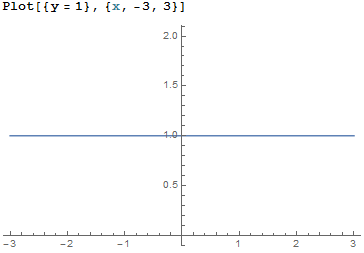
\includegraphics[height=10cm]{1.png}
 
\end{figure}

\subsection{}
Since beam $L$ parallel to the $y$-axis, $\phi+\angle LPO=\pi$. Since $\angle LPO+2\theta=\pi$, $\phi=2\theta$. Since $tan(\dfrac{\pi}{2}-\phi)=tan\angle POx=\dfrac{y}{x} $, when $\phi\neq\dfrac{\pi}{2},tan\phi=\dfrac{x}{y}$. Also the slope of the tangent line is $\dfrac{dy}{dx}$, which is also equal to $tan(\dfrac{\pi}{2}-\theta)$.

To sum up, $\phi=2\theta,tan\phi=\dfrac{x}{y},tan(\pi/2-\theta)=\dfrac{dy}{dx}$.

\subsection{}
Since the beam $L$ parallel to $y$-axis, $\theta\neq\dfrac{\pi}{2}$. So $tan\theta=\dfrac{1}{tan(\pi/2-\theta)}=\dfrac{1}{dy/dx}=\dfrac{dx}{dy}$.

To sum up, $tan\theta=\dfrac{dx}{dy}$

\subsection{}
When $\phi\neq\dfrac{\pi}{2}$,
\begin{align*}
&\phi=2\theta\\
\Rightarrow&tan\phi=tan(2\theta)=\dfrac{2tan\theta}{1-tan^2\theta}\\
\Rightarrow&\dfrac{x}{y}\Big(1-\Big(\dfrac{dx}{dy}\Big)^2\Big)=2\Big(\dfrac{dx}{dy}\Big)\\
&\Rightarrow x\Big(\dfrac{dx}{dy}\Big)^2+2y\Big(\dfrac{dx}{dy}\Big)=x
\end{align*}

When $\phi=\dfrac{\pi}{2},y=0,\theta=\dfrac{\pi}{4},\dfrac{dx}{dy}=tan(\pi/4)=1$. So $x\Big(\dfrac{dx}{dy}\Big)^2+2y\Big(\dfrac{dx}{dy}\Big)-x=x-x=0$

To sum up, the equation 
$$x\Big(\dfrac{dx}{dy}\Big)^2+2y\Big(\dfrac{dx}{dy}\Big)=x$$
always holds.


\subsection{}
Set $w=x^2$, then
\begin{align*}
&x\Big(\dfrac{dx}{dy}\Big)^2+2y\Big(\dfrac{dx}{dy}\Big)=x\\
\Rightarrow&\Big(2x\cdot \dfrac{dx}{dy}\Big)^2+4y\Big(2x\cdot \dfrac{dx}{dy}\Big)=4x^2\\
\Rightarrow&\Big(\dfrac{dw}{dx}\cdot \dfrac{dx}{dy}\Big)^2+4y\Big(\dfrac{dw}{dx}\cdot \dfrac{dx}{dy}\Big)=4w\\
\Rightarrow&w=y\Big(\dfrac{dw}{dy}\Big)+\dfrac{1}{4}\Big(\dfrac{dw}{dy}\Big)^2\\
\end{align*}
 
The straight-line solution to this equation is given by
$$w=c\cdot y+\dfrac{1}{4}c^2$$
the family of lines are parametrized by
$$\gamma(y,c)=\begin{pmatrix}
y\\c\cdot y+\dfrac{1}{4}c^2\end{pmatrix}$$
And we can obtain that
\begin{align*}
&\dfrac{\partial\gamma_1}{\partial y}\dfrac{\partial\gamma_1}{\partial c}=
\dfrac{\partial\gamma_2}{\partial y}
\dfrac{\partial\gamma_2}{\partial c}\\
\Rightarrow&1\cdot(y+0.5c)=0\\
\Rightarrow&c=-2y
\end{align*}
then $\gamma(y,c)\Big|_{c=-2y}=\begin{pmatrix}
y\\-2y\cdot y+\dfrac{1}{4}(-2y)^2\end{pmatrix}=\begin{pmatrix}
y\\-y^2\end{pmatrix}$

So the envelope of the straight line family is $w=-y^2$. While since $w=x^2$, this solution only give a point $(0,0)$ and it cannot be a solution to $x\Big(\dfrac{dx}{dy}\Big)^2+2y\Big(\dfrac{dx}{dy}\Big)=x$. 
So all possible solution to $w=y\Big(\dfrac{dw}{dy}\Big)+\dfrac{1}{4}\Big(\dfrac{dw}{dy}\Big)^2$ are 
$$w=c\cdot y+\dfrac{1}{4}c^2$$
resubstitute $w = x^2$ we can obtain that the solution to $x\Big(\dfrac{dx}{dy}\Big)^2+2y\Big(\dfrac{dx}{dy}\Big)=x$ is
$$y=c(x^2-\dfrac{1}{4c^2})\,\,\,\,\,\,,(c>0 \,\,\,according\,\,\,to\,\,\,diagram)$$

\subsection{}
Parabola can be used to focus rays into a
single point (its focus).

\section{}
\subsection{}
\begin{align*}
y_{1}(x)&=0+\int_0^x(y_0(s))^2+s^2ds
=\int_0^x(0)^2+s^2ds
=\dfrac{x^3}{3}
\end{align*}

%So $y_1(x)=\int\dfrac{x^3}{3}dx=\dfrac{x^4}{12}+C$
\begin{align*}
y_2(x)&=0+\int_0^x(y_1(s))^2+s^2ds
=\int_0^x(\dfrac{s^6}{9})+s^2ds
=\dfrac{x^7}{63}+\dfrac{x^3}{3}
\end{align*}
\begin{align*}
y_3(x)&=0+\int_0^x(y_2(s))^2+s^2ds
=\int_0^x(\dfrac{s^7}{63}+\dfrac{s^3}{3})^2+s^2ds
=\dfrac{x^{15}}{59535}+\dfrac{2x^{11}}{2079}+\dfrac{x^7}{63}+\dfrac{x^3}{3}
\end{align*}
\begin{align*}
y_4(x)&=0+\int_0^x(y_2(s))^2+s^2ds
=\int_0^x(\dfrac{s^{15}}{59535}+\dfrac{2s^{11}}{2079}+\dfrac{s^7}{63}+\dfrac{s^3}{3})^2+s^2ds\\
&=\dfrac{x^{31}}{109876902975}+\dfrac{4x^{27}}{3341878155}+\dfrac{662x^{23}}{10438212015}+\dfrac{82x^{19}}{37328445}+\dfrac{13x^{15}}{218295}+\dfrac{2x^{11}}{2079}+\dfrac{x^{7}}{63}+\dfrac{x^3}{3}
\end{align*}

\subsection{}
\begin{figure}[ht]
	\centering
	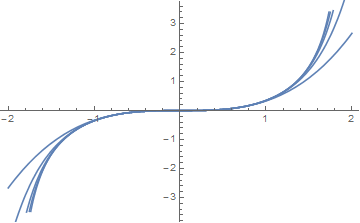
\includegraphics[height=9cm]{2.png}
	\caption{Numerical solution to (**) and $y_1,y_2,y_3,y_4$}  
\end{figure}
Since numerical solution will have great error when $x$ goes far away from 0, I just choose $[-2,2]$ to have a look.(On the right-hand side of y-axis, from the bottom to top are numerical solution, $y_4,y_3,y_2,y_1$)

\end{document}
